\documentclass[12pt, oneside]{article} 
\usepackage{amsmath, amsthm, amssymb, calrsfs, wasysym, verbatim, bbm, color, graphics, geometry, multirow}
\usepackage{graphicx}
\usepackage{tikz}
\usepackage{amsmath}
\usepackage{graphicx}
\usepackage{amsmath, amssymb, amsthm}
\usepackage{setspace}
\usepackage{tikz}
\usetikzlibrary{trees, positioning}
\usepackage{pgfplots}
\renewcommand{\baselinestretch}{1.5}
\geometry{tmargin=.75in, bmargin=.75in, lmargin=.75in, rmargin = .75in}  

\newcommand{\R}{\mathbb{R}}
\newcommand{\C}{\mathbb{C}}
\newcommand{\Z}{\mathbb{Z}}
\newcommand{\N}{\mathbb{N}}
\newcommand{\Q}{\mathbb{Q}}
\newcommand{\Cdot}{\boldsymbol{\cdot}}


\newtheorem{thm}{Theorem}
\newtheorem{defn}{Definition}
\newtheorem{conv}{Convention}
\newtheorem{rem}{Remark}
\newtheorem{lem}{Lemma}
\newtheorem{cor}{Corollary}


\title{Game Theory}
\author{Kirby CHEN}
\date{Academic Year 2024-2025}

\begin{document}

\maketitle
\tableofcontents

\vspace{.25in}

\section{Nash Equilibrium in Pure Actions}

A game is triple (I,(A$_i$), (u$_i$)) where:
\begin{itemize}
    \item I is a set of players
    \item A$_i$ is the set of actions available to player i
    \item u$_i$ is the payoff function for player i
\end{itemize}

For the moment, the functions \( u_i \) represent ordinal preferences over \( \prod_{i \in I} A_i \).

Note that we are allowing arbitrary externalities.

Consider a game with \( N \) players. A strategy profile  
\[
\mathbf{s^*} = (s_1^*, s_2^*, \dots, s_N^*)
\]  
is a \textbf{Nash equilibrium} of the game if, for every player \( i \),

\[
u_i(s_i^*, \mathbf{s}_{-i}^*) \geq u_i(s_i', \mathbf{s}_{-i}^*)
\]

Given a game \( (I, (A_i)_{i \in I}, (u_i)_{i \in I}) \), a \underline{Nash equilibrium} of this game is an \( n \)-tuple of actions \( (a^*_i)_{i \in I} \) such that for every player \( i \in I \) and for every action \( a_i \in A_i \):

\[
u_i(a^*) \geq u_i(a_i, a^*_{-i}),
\]

where \( (a_i, a^*_{-i}) \) is the list of actions that is identical to \( a^* \) except that we have replaced \( a^*_i \) by \( a_i \).

\underline{\textbf{Interpretation:}} A Nash equilibrium represents a rest point of a learning process in which each player chooses the optimal action assuming that all other players choose the same actions as in the previous period.

\underline{\textbf{Best Response}}: A strategy \( s_i \) is a best response to a strategy profile \( s_{-i} \) if it maximizes the payoff of player i given the strategies of the other players.
\[
u_i(s_i, \mathbf{s}_{-i}) \geq u_i(s_i', \mathbf{s}_{-i})
\]

\underline{\textbf{Best Response Correspondence}}: The best response correspondence of player i is the correspondence that assigns to each strategy profile \( s_{-i} \) the set of best responses of player i to \( s_{-i} \).

\subsection{Key points}
\underline{\textbf{1. Nash equilibria are fixed points of the best reply correspondence.}}

For every player \( i \in I \) define a \underline{best reply correspondence} \( BR_i : \prod_{i \in I} A_i \rightrightarrows A_i \) by setting for every \( a \in \prod_{i \in I} A_i \):

\[
BR_i(a) = \{ a_i \in A_i \mid u_i(a_i, a_{-i}) \geq u_i(a'_i, a_{-i}) \text{ for every } a'_i \in A_i \}.
\]

The \underline{best reply correspondence} \( BR : \prod_{i \in I} A_i \rightrightarrows \prod_{i \in I} A_i \) is defined by setting for every \( a \in \prod_{i \in I} A_i \):

\[
BR(a) = \prod_{i \in I} BR_i(a).
\]

By definition: \( a^* \) is a Nash equilibrium if and only if \( a^* \in BR(a^*) \), i.e., if and only if \( a^* \) is a fixed point of \( BR \).



    \section{Static Games}

\subsection{Case 1: Betrend Competition}
In betrend competition, firm face a total cost curve for producing their goods and simply choose the price for their respective goods. 
Whichever firm has the lower price will get all the customers and if the prices are the same, the customers will be split evenly.
We will assume that identical firms face a constant marginal cost c. The firms simultaneously choose their prices, p1 and p2.
let's look at it from firm 1's perspective (it will be the same for firm firm 2). 

\textbf{Firm 1 has three strategies:}

\begin{itemize}
    \item $p_1 < p_2$: Firm 1 gets all the customers and makes a profit of $p_1 - c$.
    \item $p_1 = p_2$: Firm 1 gets half the customers and makes a profit of $\frac{p_1 - c}{2}$.
    \item $p_1 > p_2$: Firm 1 gets no customers and makes a profit of 0.
\end{itemize}

Naturally, depending on what firm 2's price is, we could have any of these situations. Let s look at some different conditions.

\begin{itemize}
    \item Starting with one extreme, suppose $p_2 > p^m$, the monopoly price.
    \begin{itemize}
        \item If firm 1 chose a price above this, firm 2 would get all of the consumers since their price is lower.
        \item If firm 1 matched this price, they would get half of the consumers.
        \item If firm 1 set a price lower than this, they would get all of the consumers.
    \end{itemize}
    \item Naturally, firm 1 would actually want to set $p_1 = p^m$ in this case since that’s the price that maximizes their profit level.
\end{itemize}

\begin{itemize}
    \item Now, let’s suppose firm 2 chose some price that was at most the monopoly price, i.e., $p_2 \leq p^m$. The same results hold.
    \begin{itemize}
        \item If firm 1 chose a price above this, firm 2 would get all of the consumers since their price is lower.
        \item If firm 1 matched this price, they would get half of the consumers.
        \item If firm 1 set a price lower than this, they would get all of the consumers.
    \end{itemize}
    \item It should be obvious that firm 1 wants to set a price lower than firm 2, $p_1 < p_2$. In fact, to maximize profit, firm 1 wants to undercut firm 2 by as little as possible (a single penny). $p_1 = p_2 - \varepsilon$ where $\varepsilon > 0$ is the smallest possible number that firm 1 can pick.
    \begin{itemize}
        \item That way they get all of the customers while lowering their profit margin by as little as possible.
    \end{itemize}
\end{itemize}

\begin{itemize}
    \item Lastly, suppose firm 2's price were at or below marginal cost, $p_2 \leq c$.
    \begin{itemize}
        \item If firm 1 chose a price above this, firm 2 would get all of the consumers since their price is lower.
        \item If firm 1 matched this price, they would get half of the consumers.
        \item If firm 1 set a price lower than this, they would get all of the consumers.
    \end{itemize}
    \item Pricing below marginal cost would not be an optimal strategy for firm 1. If $p_1 < c$, firm 1 would actually lose money on each unit sold.
    \begin{itemize}
        \item Thus, the lowest (and only possible) price firm 1 is willing to charge is $p_1 = c$.
    \end{itemize}
\end{itemize}

\begin{itemize}
    \item The analysis for firm 2 is identical.
    \begin{itemize}
        \item If firm 1 prices above the monopoly price, $p_2 = p^m$.
        \item If firm 1 prices between marginal cost and the monopoly price, $p_2 = p_1 - \varepsilon$, where $\varepsilon > 0$ is the smallest possible number greater than zero.
        \item If firm 1 prices at or below marginal cost, $p_2 = c$.
    \end{itemize}
\end{itemize}

\begin{itemize}
    \item Returning to our Nash equilibrium solution concept, we know that our equilibrium is when neither firm has any incentive to deviate from their chosen strategy.
    \begin{itemize}
        \item This occurs where the best response functions intersect.
    \end{itemize}
    \item There is exactly one intersection point in the previous figure, where $p_1 = p_2 = c$. Thus, both firms price at marginal cost in equilibrium.
    \begin{itemize}
        \item This should make sense. Each firm wants to undercut the other to claim the whole market. Yet they can’t undercut anymore once the price is at marginal cost or they’ll suffer losses.
        \item Bertrand competition implies that with just two firms, we reach the perfectly competitive equilibrium.
    \end{itemize}
    \item Since price is set at marginal cost for both firms, economic profit under Bertrand competition equals zero.
\end{itemize}

\begin{figure}[h!]
    \centering
    \includegraphics[width=0.8\textwidth]{Figure/Betrend.png} % 图片文件路径
    \caption{EQ} 
    \label{fig:1} 
\end{figure}

\subsection{Case 2: Cournet Competition}

\subsection{Case 3: Stackelberg Competition}
\newpage
\section{Nash Equilibria in Mixed Actions}

\section{Incomplete Information Static Games}

\subsection{Incomplete Information}
A game has (is of) incomplete information when at least one player does not know the payoff that some player receives from some strategy profile (or terminal nodes).

In this section, we will consider simultaneously-move games with incomplete information.

As an example, consider the following game. This is a modified Prisoner’s dilemma. Prisoner 1 is not clear about the crime she committed so she doesn’t know which of the following games is played.

Prisoner 2, on the other, has more knowledge about law so he knows which game is played.

\begin{table}[h]
    \centering
    \renewcommand{\arraystretch}{1.2}
    \setlength{\tabcolsep}{8pt}
    \begin{tabular}{c c|c c|}
        \multicolumn{2}{c}{} & \multicolumn{2}{c}{\textbf{Prisoner 2}} \\
        \multicolumn{2}{c}{} & Defense & Confess \\
        \cline{2-4}
        \multirow{2}{*}{\textbf{Prisoner 1}} & Defense & -2,-2 & -10,-1 \\
        & Confess & -1,-10 & -5,-5 \\
        \cline{2-4}
        \multicolumn{4}{c}{Good}
    \end{tabular}
    \hspace{1cm}
    \begin{tabular}{c c|c c|}
        \multicolumn{2}{c}{} & \multicolumn{2}{c}{\textbf{Prisoner 2}} \\
        \multicolumn{2}{c}{} & Defense & Confess \\
        \cline{2-4}
        \multirow{2}{*}{\textbf{Prisoner 1}} & Defense & -5,-5 & -13,-4 \\
        & Confess & -4,-13 & -8,-8 \\
        \cline{2-4}
        \multicolumn{4}{c}{Bad}
    \end{tabular}
\end{table}
\break
Let's use a game tree to represent this. In the eyes of Prisoner 1, this game is like this:

\begin{center}
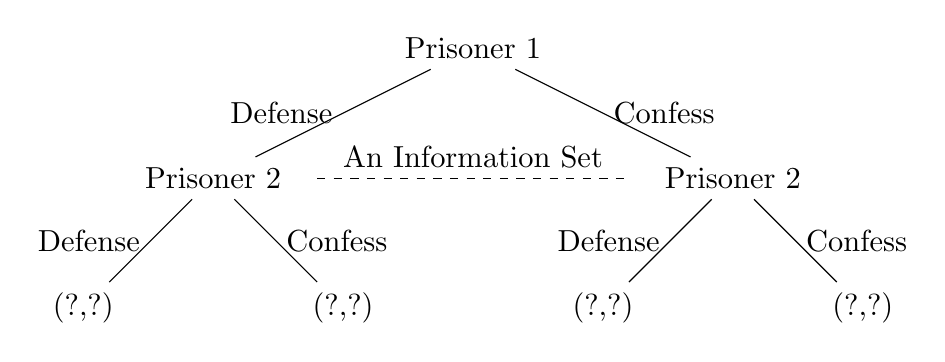
\begin{tikzpicture}[scale=1.1, transform shape]
    \tikzstyle{level 1}=[sibling distance=60mm]
    \tikzstyle{level 2}=[sibling distance=30mm]
    
    \node {Prisoner 1}
        child { node {Prisoner 2}
            child { node { (?,?) } edge from parent node[left] {Defense} }
            child { node { (?,?) } edge from parent node[right] {Confess} }
            edge from parent node[left] {Defense}
        }
        child { node {Prisoner 2}
            child { node { (?,?) } edge from parent node[left] {Defense} }
            child { node { (?,?) } edge from parent node[right] {Confess} }
            edge from parent node[right] {Confess}
        };
    
    % Drawing the information set
    \draw[dashed] (-1.8,-1.5) -- (1.8,-1.5) node[midway, above] {An Information Set};
\end{tikzpicture}
\end{center}

\subsection{Types and strategies}
Dealing with games with incomplete information is difficult. But Harsany came up with a solution to address this problem. His idea is to transform any game of incomplete information into a game with complete but imperfect information.

When doing so, we suppose the nature randomly chooses a “type” for each player. Each player knows only her own type, but not other players' type. The types of all players influence the payoff of each player.

For example, after introducing the nature and type, then we can say Prison 2 has 2 types: Good or Bad. Prisoner 2's type not only influences his own payoff, it also influences the payoff of Prisoner 1.
The game tree now looks like the following.
\begin{figure}[h!]
    \centering
    \includegraphics[width=0.8\textwidth]{Figure/incom_tree.png} 
    \caption{Incomplete Information Game Tree} 
    \label{fig:2} 
\end{figure}

\break
Prisoner 1 cannot distinguish the two decision nodes because she cannot observe the type of Prisoner 2.
Prisoner 2 has 2 types, and he can observe his own type, so he has 2 information sets.

We can still define a strategy as a function that maps an information set to a distribution over actions.
Now an information set just represents a type of a player. Here, Prisoner 1 has only one type, so she has only one information set.

Thus, we can also define a strategy as a function from a type to a distribution over action.

More formally, a static game of incomplete information can be described by:
\[
\Gamma_N = [I, \{\Delta(A_i)\}_{i \in I}, \{u_i(\cdot)\}_{i \in I}, \{\Theta_i\}_{i \in I}]
\]
such that:

\begin{enumerate}
    \item \( I \): a set of players. We assume there are \( n \) players.
    \item \( \Delta(A_i) \): the set of mixed action of player \( i \).
    \item \( \Theta_i \): a set of types of player \( i \). We define \( \Theta = \Theta_1 \times \Theta_2 \times \cdots \times \Theta_n \) and \( (\theta_i, \theta_{-i}) \) to define a type profile, where \( \theta_{-i} = (\theta_j)_{j \neq i} \).
    \item \( u_i : \prod_{j=1}^{n} \Delta(A_i) \times \prod_{j=1}^{n} \Theta_j \to \mathbb{R} \): the utility function of player \( i \), which depends on the action profile and players’ types. We use \( u_i(\alpha_1, \alpha_2, \dots, \alpha_n, \theta_1, \theta_2, \dots, \theta_n) \) to denote the expected payoff of player \( i \) when the action profile is \( (\alpha_1, \alpha_2, \dots, \alpha_n) \) and the type profile is \( (\theta_1, \theta_2, \dots, \theta_n) \).
\end{enumerate}

In the above example, \( I = \{1,2\} \), \( A_i = \{D,C\} \), \( \Theta_1 = \{\emptyset\} \) and \( \Theta_2 = \{G, B\} \). The utility function of P1 is such that \( u_1(D, D, \emptyset, G) = -2 \) and so on.

A pure strategy of player \( i \) is a function \( s_i : \Theta_i \to A_i \) such that \( s_i(\theta) \) is the action chosen by player \( i \) of type \( \theta \in \Theta_i \).

A mixed strategy of player \( i \) is a function \( \sigma_i : \Theta_i \to \Delta(A_i) \) such that \( \sigma_i(a | \theta) \) is the probability that action \( a \in A_i \) is chosen by player \( i \) of type \( \theta \in \Theta_i \). If \( A_i \) has \( m \) elements, we can also use \( \sigma_i(\theta) = (p_1, p_2, \dots, p_m) \) to represent a strategy of player \( i \) of type \( \theta \).

So for Player 1, \( s_1(\emptyset) = D \) is a pure strategy. For Player 2, \( \sigma_2(G) = \left( \frac{1}{2}, \frac{1}{2} \right) \) and \( \sigma_2(B) = (1,0) \) is a mixed strategy.

\subsection{Dominant and Dominated Strategies}
The idea of dominant and dominated strategies can be extended to an incomplete information game. We give the following definitions.

\textbf{Definition 1.} In an incomplete information game 
\[
\Gamma_N = [I, \{\Delta(A_i)\}_{i\in I}, \{u_i(\cdot)\}_{i\in I}, \{\Theta_i\}_{i\in I}],
\]
a strategy \(\sigma_i\) is said to strictly dominate \(\sigma'_i\) if for all \((\theta_i, \theta_{-i}) \in \Theta\) and all \(a_{-i} \in \prod_{j \neq i} A_j\),
\[
u_i(\sigma_i(\theta_i), a_{-i}, \theta_i, \theta_{-i}) > u_i(\sigma'_i(\theta_i), a_{-i}, \theta_i, \theta_{-i}).
\]
The strategy \(\sigma_i\) is strictly dominant if it strictly dominates every other strategy \(\alpha'_i\).

\vspace{0.5cm}

A strategy profile \((\sigma_1, \sigma_2, \dots, \sigma_n)\) is a strictly dominant strategy equilibrium if \(\sigma_i\) is a strictly dominant strategy for all \(i\).

In the previous example, regardless of the type of Player 2, for both players, Confess is a strictly dominant strategy so we can predict that both players of any type choose Confess.

The above condition is too strong. We also state a weaker one as below.

\vspace{0.5cm}

\textbf{Definition 2.} In an incomplete information game \[
\Gamma_N = [I, \{\Delta(A_i)\}_{i\in I}, \{u_i(\cdot)\}_{i\in I}, \{\Theta_i\}_{i\in I}],
\]
a strategy \(\sigma_i\) is said to weakly dominate \(\sigma'_i\) if for all \((\theta_1, \theta_2, \dots, \theta_n) \in \Theta\) and all \(a_{-i} \in \prod_{j \neq i} A_j\),
\[
u_i(\sigma_i(\theta_i), a_{-i}, \theta_i, \theta_{-i}) \geq u_i(\sigma'_i(\theta_i), a_{-i}, \theta_i, \theta_{-i})
\]
with strictly inequality for some \(a_{-i}\) and \((\theta_i, \theta_{-i})\).

The strategy \(\sigma_i\) is weakly dominant if it weakly dominates every other strategy \(\alpha'_i\).

A strategy profile \((\sigma_1, \sigma_2, \dots, \sigma_n)\) is a weakly dominant strategy equilibrium if \(\sigma_i\) is a weakly dominant strategy for all \(i\).

\subsection{Beliefs and Bayesian Games}
Now we change the payoff in the previous example a little bit. We still assume Player 1 does not know which game is played and thus is of one type, while Player 2 knows which game is played and has 2 types.

\begin{table}[h]
    \renewcommand{\arraystretch}{1.2}
    \setlength{\tabcolsep}{8pt}
    \begin{tabular}{c c|c c|}
        \multicolumn{2}{c}{} & \multicolumn{2}{c}{\textbf{Prisoner 2}} \\
        \multicolumn{2}{c}{} & Defense & Confess \\
        \cline{2-4}
        \multirow{2}{*}{\textbf{Prisoner 1}} & Defense & -2,-2 & -10,-1 \\
        & Confess & -1,-10 & -5,-5 \\
        \cline{2-4}
        \multicolumn{4}{c}{Good}
    \end{tabular}
    \hspace{1cm}
    \begin{tabular}{c c|c c|}
        \multicolumn{2}{c}{} & \multicolumn{2}{c}{\textbf{Prisoner 2}} \\
        \multicolumn{2}{c}{} & Defense & Confess \\
        \cline{2-4}
        \multirow{2}{*}{\textbf{Prisoner 1}} & Defense & -4,-5 & -8,-4 \\
        & Confess & -5,-13 & -13,-8 \\
        \cline{2-4}
        \multicolumn{4}{c}{Bad}
    \end{tabular}
\end{table}

Prisoner 1 has no dominant strategy now. If Prisoner 2's type is Good, it is optimal for Player 1 to choose Confess. If his type is Bad, it is optimal to choose Defense.

We want to have an incomplete information game version of Nash equilibrium, which we can guarantee its existence and it is an extension of the previous concepts. To do so, we will have to specify how Prisoner 1 thinks of Prisoner 2's type. Or how Prisoner 1 assigns probabilities to the two decision nodes in her information set. We introduce the following concept.

\textbf{Definition 3.} In an extensive form game \( \Gamma_E \), a belief system \( \mu : N \to [0,1] \) assigns probability to each decision node such that for any information set \( h \in H \),
\[
\sum_{x \in h} \mu(x) = 1
\]

In our example, we need to specify \( \mu(x_1) \) and \( \mu(x_2) \), the probabilities that Prisoner 1 assigns to the 2 decision nodes in her information set.

\includegraphics{Figure/incom_tree_bey.png}

To specify the beliefs of players, we usually assume the incomplete information games we consider are Bayesian games. In addition to what constitutes an incomplete information game, in a Bayesian game, nature assigns probabilities to type profiles of the players.

A Bayesian game is an incomplete information game with a probability distribution \( p \) over type profiles \( \Theta = \Theta_1 \times \Theta_2 \times \cdots \times \Theta_n \). We assume this distribution \( p \) is a common knowledge.

When each player has finite types, we use a probability mass function \( p \) such that \( p(\theta_1, \theta_2, \dots, \theta_n) \) is the probability the nature assigns to type profile \( (\theta_1, \theta_2, \dots, \theta_n) \). When types are real numbers, \( p \) is the probability density function.

We use 
\[
\Gamma_N = [I, \{\Delta(A_i)\}_{i\in I}, \{u_i(\cdot)\}_{i\in I}, \{\Theta_i\}_{i\in I}, p(\cdot)]
\]
to represent a Bayesian game.

In the previous example, we can assume the nature assigns probability \( p(\emptyset, G) \) to type profile \( (\emptyset, G) \), and assigns probability \( p(\emptyset, B) \) to type profile \( (\emptyset, B) \). The game tree thus looks like the following.


\includegraphics{Figure/incom_tree_bey2.png}
\textit{p} is called the prior belief in the sense that players know this even without knowing their own types. But after observing \( \theta_i \), player \( i \) will update her belief using Bayes rule. She will assign belief to \( (\theta_i, \theta_{-i}) \) conditional on \( \theta_i \). In notation, that is

\[
p(\theta_i, \theta_{-i} | \theta_i) = \frac{p(\theta_i, \theta_{-i})}{\sum_{\theta'_{-i}} p(\theta_i, \theta'_{-i})}
\]

This is called the posterior belief of player \( i \) of type \( \theta_i \).

Now we update the belief of Prisoner 1. This is trivial because Prisoner 1 has only one type.

\[
p(\emptyset, B | \emptyset) = \frac{p(\emptyset, B)}{p(\emptyset, B) + p(\emptyset, G)} = p(\emptyset, B)
\]

This is the probability that Prisoner 1 assigns to \( x_2 \) in her information set.

\[
\mu(x_2) = p(\emptyset, B)
\]

We call \( p(\cdot) \) the prior belief, which is the belief of a player when she has not observed her type yet. We call \( p(\cdot | \theta_i) \) the posterior belief of player \( i \), which is the belief of her after she observed her type.

\end{document}
